\chapter{\textbf{Requirements Analysis}}\label{grundlagen}
In order to select the most suitable technologies and design the system, it is first necessary to establish clear requirements. In this chapter, the aforementioned requirements will be enumerated and elucidated.
In order to maintain consistency regarding the compliance level, the terms "must," "should," and "will" were employed.
The following words shall be explained in brief. The term "must" is employed to signify an unconditional obligation, implying that the fulfillment of this requirement is not subject to discussion or negotiation. The term "should" conveys a degree of desirability, indicating that fulfillment of the requirement would be advantageous. The term "will" signifies that this particular requirement is currently under consideration for inclusion in the subsequent release. However, it is imperative to maintain awareness of this requirement so that the system can be designed in a manner that facilitates its seamless integration in the future.
\subsection{Functional System Requirements} % (from your requirements table)
\begin{tabularx}{\textwidth}{|X|X|}
	\hline
\textbf{Requirement}	& \textbf{Explanation} \\
	\hline
The system must show KPIs that are relevant for the sewing process	&  In the workshops there must be some KPIs that fit into the story of a textile production with a sewing process\\
	\hline
The system should show aditional KPIs that are relevant for the manufacturing industry in general	&  Workshop participants are from all sorts of companies within the manufacturing industry\\
	\hline
 The system must present these KPIs in a visual manner that provides information about the classification of the current value e.g. with colors and thresholds	& So that the management can act quickly upon the KPIs and does not need to lookup thresholds \\
	\hline
The system must provide the user with the ability to change the timeframe on which the KPIs are calculated	&  Especially when looking at historic data it is usefull to be able to set the timeframe\\
	\hline
The system should show graphs with historical data & Enables management to see trends and patterns\\
	\hline
\end{tabularx}

\subsection{Non-Functional Requirements} %(scalability, security, real-time processing)
\begin{tabularx}{\textwidth}{|X|X|}
	\hline
\textbf{Requirement}	&  \textbf{Explanation}\\
	\hline
The system must make use of open source software where possible	&  To be replecable by small and medium companies\\
	\hline
The system must be capable to generate all of the KPIs from the machine-data without installing any additional sensors	&  \\
	\hline
The system must be designed in a way that makes it easily scalable	&  Usually more than just one machine need to be considered for monitoring\\
	\hline
The system must be deployable with minimal effort	&  To be able to deploy elsewhere with not much effort \\
	\hline
The system must be capable to retrieve raw data via opc-ua	&  The PLC to which the sewing machine is connected publishes the data over opc-ua\\
	\hline
The system should make use of existing patterns, frameworks and solutions were possible	&  The system shall serve as a reference for other systems that are more readily implementable\\
	\hline
The system should update the KPIs in real-time (<10s)	&  To support timely interventions\\
	\hline
 The system must be able to run on a local machine and therefore independent of any cloud service	&  \\
	\hline
The system must provide the user with the ability to access the dashboard from within the shopfloor network	&  \\
	\hline
\end{tabularx}

\subsection{IoT Platform Evaluation and Selection} 
The raw data from the PLC had to undergo processing, storage, and visualization. The utility of IoT platforms stems from their ability to execute these functions and frequently extend beyond them.  These systems meet the criteria for scalability and leverage existing solutions. To ensure that the selected platform satisfies other requirements and does not conflict with any necessary ones, a decision support framework was developed. The present framework draws inspiration from the one proposed by Gustin and Jasperneite \cite{gustinIoTDeviceManagement2022}. The researchers identified a set of criteria and classified them into categories. The categories encompassed "Knock-Out," "Device Management," "Hosting," "General," and "Effort." Each category was assigned a weight, with the exception of the "Knock-Out" category. The "Knock-Out" category indicates that a criterion tagged with it must be met; otherwise, the platform will not be considered further. The weights are expressed as percentages, and when added together, they equal 100\%. In addition, each criterion is assigned a distinct weight, thereby enabling the allocation of greater significance to specific criteria. The evaluation of each platform is subsequently determined by the following formula:
\[ s_i = f_i \cdot 100P \cdot \mathit{weight}_{category} \cdot \mathit{weight}_{criterion} \]
In this context, $f_i$ denotes the fulfillment factor.
The newly developed framework is distinguished by the following characteristics: The criteria are flexible and should be altered according to the requirements. The aforementioned study concentrates on device management; however, this is not a salient issue in the context of the proposed system. The categories were modified to "Knock-Out," "High Importance," "Mid Importance," and "Low Importance." In this manner, the criteria are not constrained to a particular subject matter; rather, they can be assigned an extent of importance at will. The numerical values assigned to the categories are as follows: 1 for low importance, 2 for medium importance, and 3 for high importance. The new formula for calculating the platforms' score is more straightforward as well:
\[ s_i = f_i \cdot \mathit{weight}_{category} \]
The fulfillment factor is typically binary in nature. The value of the variable can be either one or zero; however, in some cases, it can also be fractional. For instance, it would be advantageous for the platforms to support additional communication protocols beyond OPC UA. Specifically, the focus is on HTTP, MQTT, CoAP, and AMQP. In the event that a given platform offers support for only one of these, it is awarded a quarter point. In the event that this is the case, it will be elucidated in the subsequent explanation. The fulfillment of the criteria was determined in the same manner as that employed by the researchers. An investigation was conducted into the documentation, website, and GitHub repository of the platform. In the event that information regarding the availability of the criterion was ascertained, the point was granted. In the absence of pertinent information, the concept in question was deemed to be nonexistent.
The subsequent paragraphs will provide detailed explanations for each of the aforementioned criteria. A selection of the materials was obtained from the publication by Gustin and Jasperneite if their utility was deemed to be beneficial. The remaining ones were developed in response to specific requirements.

\subsubsection{Knock-Out Criteria}
\textbf{Availability of Documentation}\\
The implementation, deployment, and utilization of the solution are contingent upon the availability of English-language documentation, which is imperative for effective operation. This criterion originates from the seminal contributions of  Gustin and Jasperneite\\
\textbf{Cloud independence}\\
In order to guarantee that the platform can be hosted on a local server that is accessible via the shopfloor network and that no additional cloud services are required, this criterion was established. This criterion is derived directly from the stipulated requirements.\\
\textbf{Ability to process raw data and derive KPI's from it}\\
In order to visualize the KPIs, the data must first undergo processing, after which the KPIs are to be calculated based on the processed data. This criterion pertains to the requirement of calculating KPIs. \\
\textbf{OPC-UA capability}\\
The PLC that controls the sewing machine transmits the data via the OPC UA protocol. Therefore, it is imperative that the platform demonstrate its capacity to effectively manage this particular protocol. This criterion is predicated on the requirements.

\subsubsection{High Importance Criteria}
\textbf{Dashboarding Capabilities}\\
In order to facilitate the visualization of KPIs, the platform must possess the capacity to construct dashboards. This criterion pertains to the necessity of possessing the capacity for visualizing KPIs.\\
\textbf{Actively Maintained}\\
This criterion is instrumental in ensuring the platform's security and compatibility with evolving technologies and standards.The necessity for this criterion arises from the imperative for open-source software.\\
\textbf{Completion of Server SW}\\
This criterion offers insight into the ease with which the software can be installed. A score of one is assigned if a Docker image is provided, and a score of zero is assigned if only source code is available. This criterion is derived from the work of Gustin and Jasperneite\\
\textbf{Development of the server-side application}\\
This criterion delineates the ease with which rules can be created and data processed within the application. In the event that a rule engine (low code) is provided, a point will be awarded. In the event that an SDK is provided, a total of 0.5 points will be allotted. This criterion originates from the work of Gustin and Jasperneite\\
\textbf{Examples for Server-side implementation}\\
These examples methodically illustrate the server-side implementation process and the anticipated outcomes.This approach has been shown to expedite the implementation process.
This criterion originates from the work of Gustin and Jasperneite

\subsubsection{Medium Importance Criteria}
\textbf{Supports MQTT, HTTP, CoAP, AMQP}\\
The implementation of these protocols would significantly augment the system's scalability, as it would facilitate the connection of a greater number of machines, gateways, and microcontrollers. This criterion pertains to the necessity of having a scalable system with minimal effort.\\
\textbf{Availability of Tutorials}\\
Tutorials are instrumental in facilitating user comprehension of the platform and its applications, thereby accelerating the development process. This criterion originates from the work of Gustin and Jasperneite

\subsubsection{Low Importance Criteria}
\textbf{Fault Detection}\\
This feature facilitates the collection of data pertaining to anomalous behavior or fault conditions of the machine. Therefore, it facilitates the identification and resolution of potential issues. While it would certainly be a beneficial addition, this feature does not directly align with the primary objectives of the system.
This criterion is derived from the work of Gustin and Jasperneite\\
\textbf{Heartbeat Monitor}\\
This feature periodically ascertains the online status of the connected machine. Consequently, this would facilitate the identification of device connectivity issues and ensure system reliability.
This feature is commendable, yet it does not directly align with the primary function of the system.
This criterion is derived from the work of Gustin and Jasperneite\\\\


The  platforms to be evaluated were derived from two papers that themselves evaluated IoT platforms. Initially, the open-source platforms from the aforementioned study were selected. These include openBalen, Thingsboard, Kapua, OpenRemote, Ubuntu Core, FIWARE, OpenMTC, Mainflux, and DeviceHive. In a separate study, Turki's 2024 investigation {\cite{turkiEvaluatingOpenSource2024} focused exclusively on the evaluation of open-source Internet of Things (IoT) platforms, utilizing data derived from GitHub statistics. The following factors were taken into consideration: the stars that were given by users, health, contributors, open issues, closed issues, and releases. Due to the more objective nature of this evaluation, only the top five IoT platforms were selected. The restriction to a specific number was necessitated by the impracticality of evaluating an indefinite number of platforms, as this would have entailed an inordinate amount of time. The top five platforms identified in this study are Thingsboard, Digiot, Mainflux, OpenRemote, and IotSharp.  However, it should be noted that only two of these findings were in disjunction with those selected from Gustin and Jasperneite's work. In the course of the research, the Node-RED platform emerged on a regular basis; however, it was not referenced in the evaluated documents. The platform was also mentioned by a colleague, and it was therefore given due consideration. Additionally, UMH was selected for evaluation because it builds upon robust open-source tools, such as Grafana and Apache Kafka, and supports a wide array of protocols.\\
The ensuing table 4.1 presents the results of the aforementioned calculations. It is imperative to note that only the platforms that met all of the Knock-Out criteria are displayed therein.\\

\begin{table}[H]
	%\toprule
	\caption{IoT Platform Evaluation}
	\label{tab:platform-evaluation}
	\centering
	\begin{tabu}{l @{\hspace{2cm}} r}
		\textbf{IoT Platform} & \textbf{Score} \\
		\midrule
		Thingsboard  & 19.5 \\
		Node-Red     & 21.5 \\
		FIWARE       & 19.0 \\
		OpenRemote   & 12.0 \\
		UMH          & 20.5 \\
		\bottomrule
	\end{tabu}
\end{table}

The evaluation metrics for Node-RED, ThingsBoard, and UMH exhibited a high degree of similarity, suggesting comparable levels of suitability among these options. Consequently, an in-depth investigation was conducted to ascertain their system requirements. Of the three options, the UMH configuration exhibits the most demanding specifications. It requires 200 GB of persistent memory, 16 GB of RAM, and an 8-core CPU \cite{UMHInstallationRequirements}, all of which the server configuration is incapable of meeting. The server configuration, on the other hand, has a specification of 100 GB of persistent memory, 8 GB of RAM, and an 8-core CPU. In the context of Thingsboard, the minimum amount of RAM required is specified as 4 GB \cite{thingsboardInstallingThingsBoardCE}. According to the official Node-RED website, there are no listed system requirements. However, it has been documented that it is capable of operating on a Raspberry Pi \cite{RunningNodeREDLocally}. Additionally, certain users have attested to the successful execution of the program on a Raspberry Pi 2 model \cite{NodeRedMinimun2020}, which possesses a mere 1 GB of RAM and a 900 MHz quad-core central processing unit  \cite{ltdBuyRaspberryPi}. Given its ostensibly minimal complexity and superior performance metrics in the preliminary evaluation, Node-RED was designated as the IoT platform for the system under development.

\subsection{Database Selection}
The selection of a suitable DBMS was imperative for the storage of the data. In the theoretical foundations, the rationale for the superiority of a time series database in the context of IoT streaming data over a relational database was previously delineated. The selection of the Timeseries Database Management System (TS-DBMS) was executed with a lower degree of sophistication compared to that of the IoT Platform. The rationale underlying this matter is predicated upon the temporal limitations imposed on the undertaking. A comprehensive investigation was conducted to ascertain the most prominent TS-DBMSs on db-engines.com, a website dedicated to determining the popularity of DBMSs. The following metrics have been identified as contributing factors to the popularity ranking:

\begin{itemize}
	\item The number of mentions on websites
	\item General intrest in the system using Google Trends
	\item The number of related questions and posts on well-known IT Q\&A sites
	\item The number of job offers in which the system was mentioned
	\item The number of mentions on professional networks
	\item The number of mentions on social networks
\end{itemize}

Subsequently, the capacity of InfluxDB to process boolean values was ascertained. This assertion was corroborated in the documentation \cite{WriteDataInfluxDB}. In addition, an assessment was conducted to ascertain whether InfluxDB is compatible with Node-RED. The package that was found (node-red-contrib-influxdb 0.7.0) has been determined to only support InfluxDB 1.x and 2.0 \cite{Noderedcontribinfluxdb}. Prior to this, it was determined that InfluxDB 3 Core's capacity for querying data is confined to a span of merely 72 hours \cite{QueryDataGet}, a limitation that was deemed inadequate in view of the necessity to compute historical KPIs. Consequently, InfluxdDB v2 was selected due to its compatibility with Node-RED and its capacity to support unlimited querying windows.

\subsection{Dashboarding Tool Selection}
Initially, the objective was to leverage the dashboarding capabilities of the selected IoT Platform Node-RED.
However, it appears that the utilization of this particular node-RED feature for visualization purposes is not a prevalent practice. In contrast, another software program, Grafana, was utilized in a significant number of cases similar to the one under consideration in this study. Consequently, the decision was made to utilize Grafana for the development of dashboards, with the objective of facilitating the visualization of the KPIs. This approach was adopted to enhance the probability that other colleagues would be acquainted with the solution, thereby facilitating a more streamlined handover process. The decision was further corroborated by Rani in his work \cite{raniToolsTechniquesRealtime2025}, who states that it is highly appropriate for time series visualization and monitoring. Additionally, the integration of the system with various databases, including InfluxDB, is emphasized.

\subsection{System Architecture}
The system architecture was designed in accordance with the three-tier architecture pattern from the IIRA mentioned in the foundation chapter. The Three Tier Architecture Pattern was selected because it exhibits a clear separation of concerns between the edge, platform, and enterprise tiers, thereby facilitating enhanced maintainability. Additionally, the progression of the distinct components is rendered more straightforward and less susceptible to errors in comparison to a monolithic application. The selected architecture pattern offers a distinct advantage, namely the seamless integration of supplementary devices and services. The incorporation of devices into the Node-RED system is contingent upon their connectivity to the shopfloor network. The integration of services at the platform or enterprise tier can be accomplished without the need for significant alterations to the existing system, thereby facilitating flexible expansion and adaptation to novel requirements.
\begin{figure}[H]
	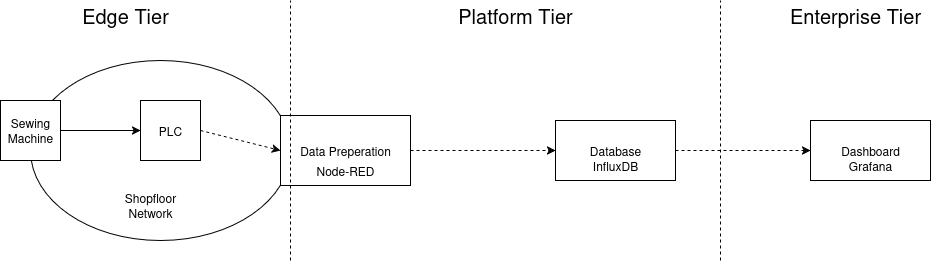
\includegraphics[width=\linewidth]{pic/system_overview.png}
	\caption{System Architecture}
	\label{fig:Model-Component-Pattern}
\end{figure}
The signal outputs from the sewing machines are wired to the PLC, as illustrated by the continuous line. Conversely, the dashed lines signify the transmission of data either over a network or within a server. The PLC provides these signals via OPC UA, and it is accessible via the shopfloor network. In the context of this architecture, Node-RED performs a variety of functions. Initially, it functions as an IoT gateway, thereby aggregating data from disparate sources. In this particular instance, the sole source of data is from the PLC. However, the component is also capable of performing data processing operations.  Subsequently, the data is transmitted to the database. From there, it can be queried with the dashboarding solution. 


\subsection{KPI Selection and Justification}
The selection of KPIs is contingent upon the fulfillment of two requirements. First, it is necessary to establish a set of KPIs that are pertinent to the sewing process. Secondly, it is imperative to establish KPIs that are pertinent to manufacturing companies in general. Additionally, it is imperative that these KPIs be computable based on the available signals. Therefore, the initial step was to ascertain which elements that provide support can be calculated based on the signals. In addition, a determination was made regarding the observations that can be derived from the available signals. It is imperative to acknowledge that merely four of the machine's signals are accessible.

Based on the analysis of the available machine signals—namely, thread trimming, pressure foot position, and main shaft rotation—a distinct production pattern can be identified and quantified. The observed sequence is as follows:

Initially, the pressure foot is lifted to allow the operator to insert the material. Subsequently, the pressure foot is lowered, securing the material in place. The sewing process then Beginnt, as indicated by the activation of the main shaft rotation signal. This signal remains true for the duration of the seam and returns to false upon completion. Following this, the pressure foot is raised again to facilitate removal of the finished workpiece. During this interval, the thread trimming signal is activated, indicating that the thread is being cut. Finally, the pressure foot is lowered once more, marking the conclusion of the production cycle.

According to the established sequence of events, the duration of the machine's operational time can be determined. The duration of the main shaft rotation signal being true corresponds to the actual sewing time. The number of pieces produced can be determined by counting the instances in which the thread trimming signal transitions to true, as each event signifies the completion of a workpiece. Furthermore, the cycle time can be calculated by measuring the interval between consecutive activations of the thread trimming signal.
The signal "other than homescreen" could be indicative of a modification in the machine's configuration.
The signal "homescreen and not sewing" can be used to observe the machine's activation. One might hypothesize that this phenomenon is merely an inverted state of the "upper shaft rotating" signal. This phenomenon is observed when the machine is activated. However, when the machine is deactivated, all signals are false. Therefore, the transition from all signals being false to "homescreen and not sewing" being true, while the other signals remain false, would indicate the activation of the machine. This could be used to measure setup time until the first pattern arises.
When only the "homescreen and not sewing" signal is active, it means the machine is idle. Therefore, the length of time that the machine is in the idle state can be measured.

\subsubsection{Supporting Elements}
To facilitate a comprehensive understanding of the supporting elements and the KPIs, the following section provides detailed explanations of these elements, along with their respective formulae if the calculation involves more the simply counting or measuring. Most of the definitions stem from Kang et al. \cite{kangHierarchicalStructureKey2016} Hierachical Structure of Key Performance Indicators [...].\\

\textbf{Processed Quantity (PQ)}
The production of a piece is initiated with the trimming of the thread. The calculation of the pieces is achieved through the enumeration of these events.\\
\textbf{Planned Downtime (PDT)}
In accordance with standard practice, the planned downtime is intended to encompass deliberate maintenance procedures and related activities. However, in the absence of such scheduled maintenance, the only components that are considered to be within the scope of planned downtime are the designated breaks. While it does not technically constitute a form of downtime, for the sake of illustration, the aforementioned period will be designated as "downtime." \\
\textbf{Planned Operation Time (POT)}
The designated period when a machine is available for use. \\
\textbf{Actual Down Time (ADT)}
The actual duration during which production is suspended due to breakdowns, brief stoppages, and other unanticipated disruptions.\\
\textbf{Actual Production Time (APT)}
The period during which the machine is actively producing for an order, encompassing only value-adding activities.
In the instance of the production pattern, the worker is engaged in the active utilization of the machine. The calculation of production time is determined by the summation of the duration of these patterns.\\
\textbf{Planned Cycle Time (PCT)}
The estimated ideal time required to manufacture a single unit. The cycle time is defined as the time interval between the completion of one task and the commencement of the next. In this work the cycle time is only measuring the single step undertaken on the sewing machine under consideration. Kang et al. designate it "planned run time per item." However, given the significance of this metric for sewing-specific processes, it is referred to as "cycle time" in accordance with sewing-related publications.\\
\textbf{Actual Cycle Time (ACT)}
The actual time required to manufacture a single unit.\\
\textbf{Setup Time (ST)}
This period is typically characterized by the machine's preparation for the subsequent order. In this study, the setup time is defined as the interval between the initiation of the machine at the commencement of a shift and the first production of a piece. This specific definition is employed due to the inherent limitations of the measurement capability, which restricts the evaluation to this particular temporal interval.\\
\textbf{Idle Time (IT)}
The time during which the machine could potentially be utilized but is not being actively employed.\\
\textbf{Planned Busy Time (PBT)}
The scheduled period during which a machine is actively engaged in operation.

\subsubsection{Maintenance Elements}
\textbf{Time to Repair (TTR)}
The period during which a machine is rendered inoperable due to a malfunction, i.e., undergoing maintenance or repair.\\
\textbf{Time to Failure (TTF)}
The period during which a machine is operational, commencing at the conclusion of the repair process and concluding when the machine experiences a subsequent failure.\\
\textbf{Operating Time between Failures (OTBF)}
The effective production time of a unit measured between two successive instances of machine failure.\\
\textbf{Failure Events (FE)}
The total count of occurrences during which the machine was non-operational.

\subsubsection{Basic KPIs}
The supporting elements that have been explained are used to calculate the basic KPIs.
Some of these KPIs were mentioned in studies on sewing performance measurement. These are performance, availability, OEE and average cycle time. However, these KPIs are not only interesting for the textile industry because they are also generally relevant to production. Some other KPIs are simply averages of supporting elements. They help identify the reasons behind the values of higher-level KPIs. Each of the selected KPIs will now be explained and shown with its respective formula.\\
\\
\textbf{Performance}\\
The performance rate is a KPI which is necessary to calculate overall equipment effectiveness (OEE). It measures the speed at which equipment operates. It is compared to the equipment's maximum operating speed because this comparison is necessary to determine the equipment's effectiveness. \cite{muchiriPerformanceMeasurementUsing2008}
\[
\text{Performance Efficiency (P)} = \frac{\text{Theoretical Cycle time (hrs)} \times \text{Produced Pieces}}{\text{Operating Time (hrs)}}
\]
The term "actual output" refers to the number of units that are produced during the operation, whereas "theoretical cycle time" signifies the minimum potential cycle time that could have been achieved at the fastest practical speed. Operating time is defined as the duration during which the machine is in active operation.\\
\textbf{Availability}
is defined as the ratio between the actual production time and the planned busy (production) time.
\[
\text{Availability} = \frac{\text{Actual Production Time}}{\text{Planned Busy Time}}
\]
\textbf{Quality}
This KPI is defined as the proportion of high-quality products in relation to the total number of units produced.
\[
\text{Quality Rate (Q)} = \frac{\text{(Total Production - Defect Amount)}}{\text{Total Production (Units)}} \times 100
\]







